\documentclass[a4paper, 12pt]{article}
\usepackage[utf8]{inputenc}
\usepackage[english, russian]{babel} 
\usepackage[left = 3cm, right = 1cm, top = 2cm, bottom = 2cm]{geometry};
\usepackage{mathtools, graphicx}
\usepackage{amssymb}

\linespread{1.25}

\title{ДЗ № 1: Регулярные языки и конечные автоматы.}
\author{Никогосян Шираз. Группа А-13б-19.}
\date{}

\begin{document}

\maketitle

\newpage

\section{Задание № 1.  Построить конечный автомат, распознающий язык.}

Ответом на данное задание является конечный автомат, распознающий описанный язык. Автомат должен быть детерминированным.

\begin{enumerate}

\item$$ L = \{\omega \in \{a, b, c\}^* \mid  |\omega|_c = 1 \} $$
\begin{figure}[!h]
\centering
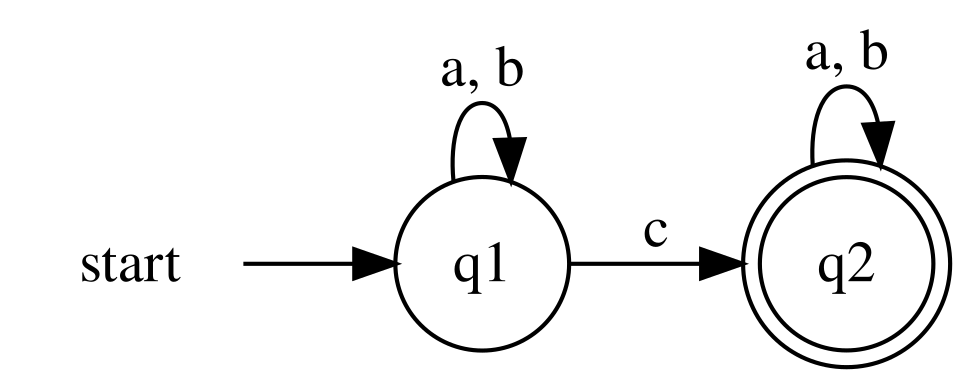
\includegraphics[scale = 1]{Task_1_1.png}
\caption{Задание № 1.1.}
\end{figure}

\item$$ L = \{\omega \in \{a, b\}^* \mid |\omega|_a \leq 2,|\omega|_b \geq 2 \} $$
\noindentДанный язык состоит из слов, в которых могут встретиться 1 или 2 буквы <<a>> и бесконечное количество букв <<b>>, начиная с 2-х. Рассмотрим каждое из условий по отдельности.

\noindentПусть автомат A распознает следующий язык: $ L_1 = \{\omega \in \{a, b\}^* \mid |\omega|_a \leq 2 \} $
\begin{figure}[h!]
\centering
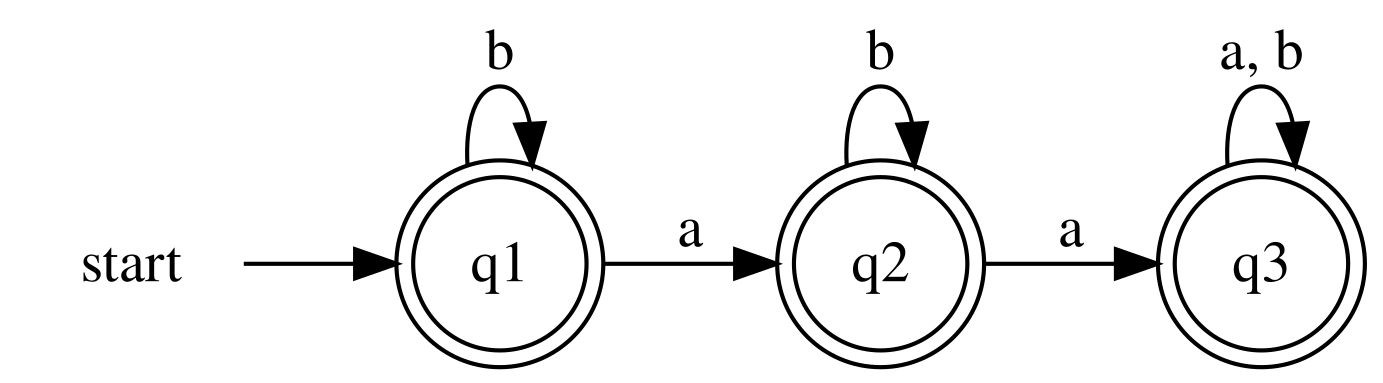
\includegraphics[scale = 1]{Task_1_21.png}
\caption{Задание № 1.2. Автомат A.}
\end{figure}

\noindentПусть автомат B распознает следующий язык: $ L_2 = \{\omega \in \{a, b\}^* \mid |\omega|_b \geq 2 \} $
\begin{figure}[!h]
\centering
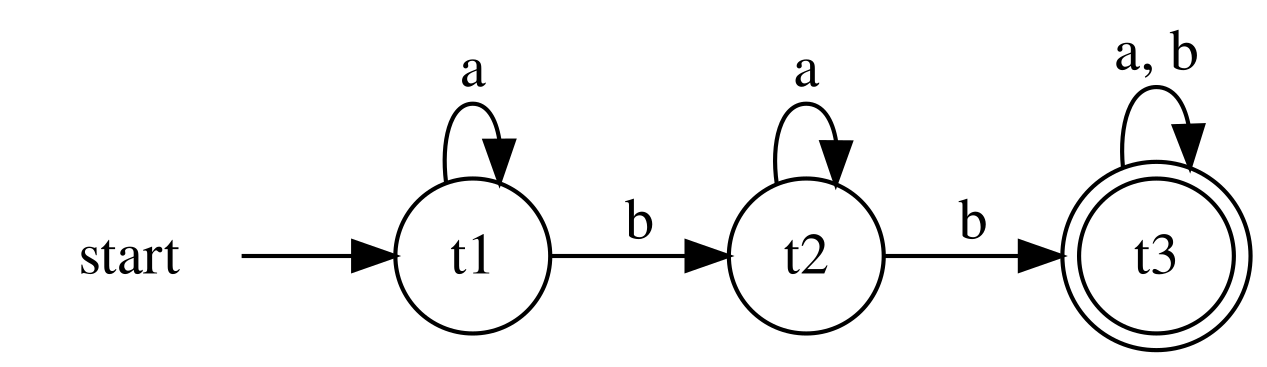
\includegraphics[scale = 0.7]{Task_1_22.png}
\caption{Задание № 1.2. Автомат B.}
\end{figure}

\noindentАвтомат A: $ \Sigma_1 = \{a, b\}$, $ Q_1 = \{q1, q2, q3 \} $, q1 - н.ч., $ T_1 = \{q1, q2, q3 \} $, $ \delta_1 $ - ф.п.

\noindentАвтомат B: $ \Sigma_2 = \{a, b\}$, $ Q_2 = \{t1, t2, t3 \} $, t1 - н.ч., $ T_2 = \{t3 \} $, $ \delta_2 $ - ф.п.

\noindentРассмотрим прямое произведение 2-х автоматов.

\noindent$ \Sigma = \{a, b\}$

\noindent$ Q = \{q1t1, q1t2, q1t3, q2t1, q2t2, q2t3, q3t1, q3t2, q3t3 \} $

\noindentНачальное состояние = q1t1

\noindent$ T = \{q1t3, q2t3, q3t3 \} $

\begin{center}
\begin{tabular}{ |c|c|c| } 
\hline
\, & a & b \\
\hline
 q1t1 & q2t1 & q1t2 \\
\hline
q1t2 & q2t2 & q1t3 \\
\hline
q1t3& q2t3 & q1t3 \\
\hline
q2t1 & q3t1 & q2t2 \\
\hline
q2t2 & q3t2 & q2t3 \\
\hline
q2t3 & q3t3 & q2t3 \\
\hline
q3t1 & - & q3t2 \\
\hline
q3t2 & - & q3t3 \\
\hline
q3t3 & - & q3t3 \\
\hline
\end{tabular}
\end{center}

\begin{figure}[!h]
\centering
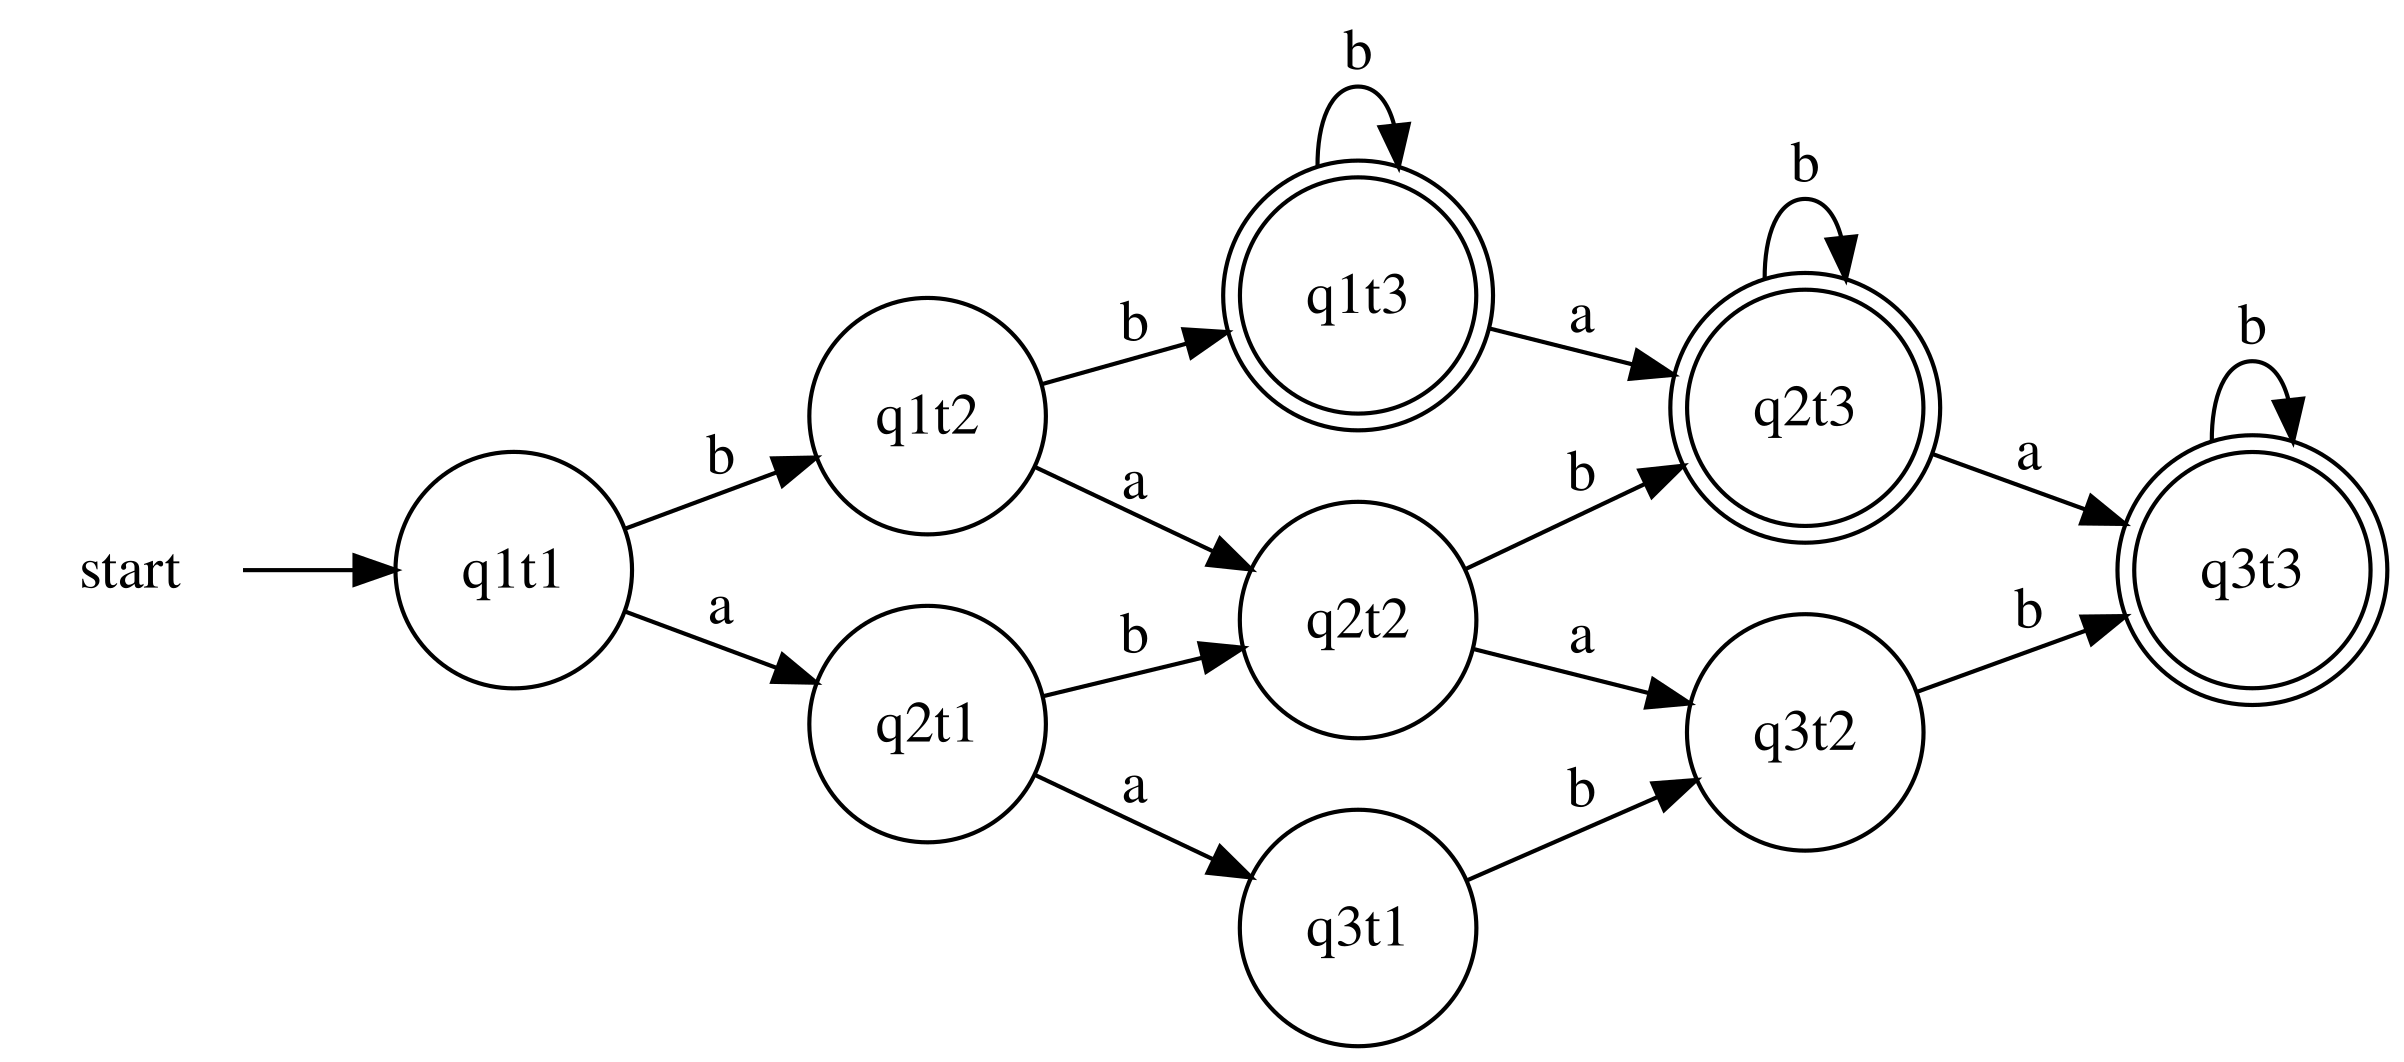
\includegraphics[scale = 0.8]{Task_1_2.png}
\caption{Задание № 1.2. Итоговый автомат.}
\end{figure}

\item$$ L = \{\omega \in \{a, b\}^* \mid |\omega|_a \neq |\omega|_b \} $$

\noindentЭтот язык нельзя описать с помощью ДКА, т.к. для распознования данного языка требуется запоминать количество символов. Язык L является не регулярным языком.

\item$$ L = \{\omega \in \{a, b\}^* \mid \omega\omega = \omega\omega\omega \} $$
\noindentДанных язык состоит только из пустых слов.
\begin{figure}[!h]
\centering
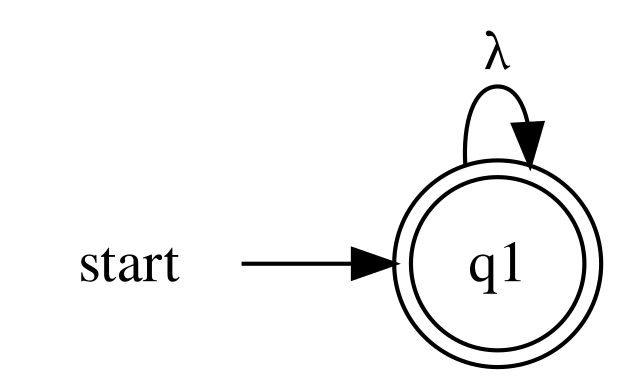
\includegraphics[scale = 1]{Task_1_4.png}
\caption{Задание № 1.4.}
\end{figure}

\end{enumerate}

\section{Задание № 2. Построить конечный автомат, используя прямое произведение.}

Ответом на данное задание является конечный автомат, распознающий описанный язык. Требуется, чтобы он был построен при помощи прямого произведения ДКА и его свойств.

\begin{enumerate}

\item$$ L_1 = \{\omega \in \{a, b\}^* \mid |\omega|_a \geq 2 \wedge |\omega|_b \geq 2 \} $$

\noindentПусть автомат A распознает следующий язык: $ L_{11} = \{\omega \in \{a, b\}^* \mid |\omega|_a \geq 2 \} $
\begin{figure}[!h]
\centering
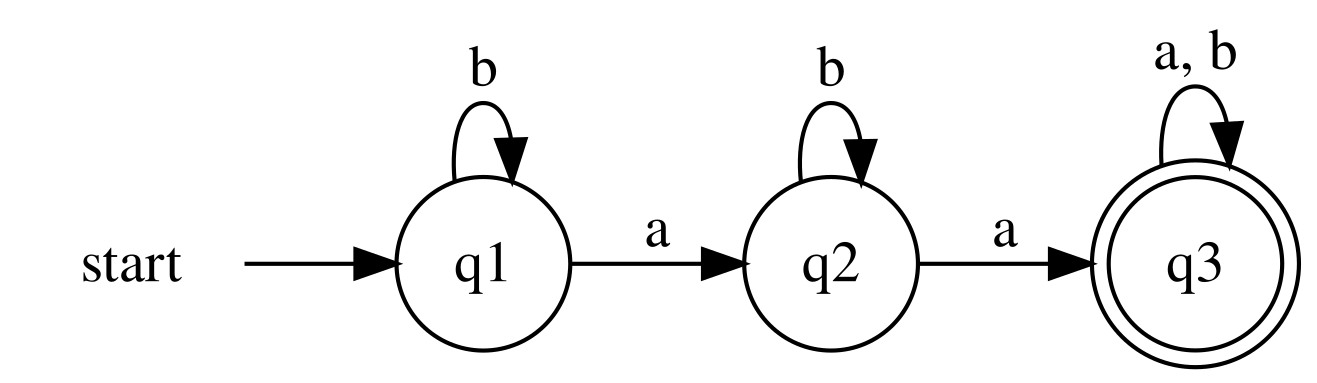
\includegraphics[scale = 1]{Task_2_11.png}
\caption{Задание № 2.1. Автомат A.}
\end{figure}

\noindentПусть автомат B распознает следующий язык: $ L_{12} = \{\omega \in \{a, b\}^* \mid |\omega|_b \geq 2 \} $
\begin{figure}[!h]
\centering
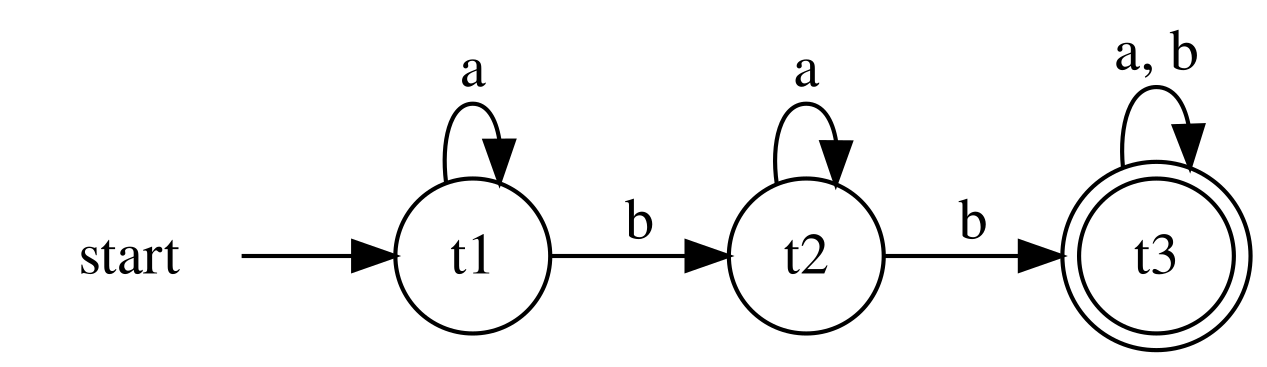
\includegraphics[scale = 1]{Task_2_12.png}
\caption{Задание № 2.1. Автомат B.}
\end{figure}

\noindentАвтомат A: $ \Sigma_1 = \{a, b\}$, $ Q_1 = \{q1, q2, q3 \} $, q1 - н.ч., $ T_1 = \{q3 \} $, $ \delta_1 $ - ф.п.

\noindentАвтомат B: $ \Sigma_2 = \{a, b\}$, $ Q_2 = \{t1, t2, t3 \} $, t1 - н.ч., $ T_2 = \{t3 \} $, $ \delta_2 $ - ф.п.

\noindentРассмотрим прямое произведение 2-х автоматов.

\noindent$ \Sigma = \{a, b\}$

\noindent$ Q = \{q1t1, q1t2, q1t3, q2t1, q2t2, q2t3, q3t1, q3t2, q3t3 \} $

\noindentНачальное состояние = q1t1

\noindent$ T = \{q3t3 \} $

\begin{center}
\begin{tabular}{ |c|c|c| } 
\hline
\, & a & b \\
\hline
 q1t1 & q2t1 & q1t2 \\
\hline
q1t2 & q2t2 & q1t3 \\
\hline
q1t3& q2t3 & q1t3 \\
\hline
q2t1 & q3t1 & q2t2 \\
\hline
q2t2 & q3t2 & q2t3 \\
\hline
q2t3 & q3t3 & q2t3 \\
\hline
q3t1 & q3t1 & q3t2 \\
\hline
q3t2 & q3t2 & q3t3 \\
\hline
q3t3 & q3t3 & q3t3 \\
\hline
\end{tabular}
\end{center}

\begin{figure}[!h]
\centering
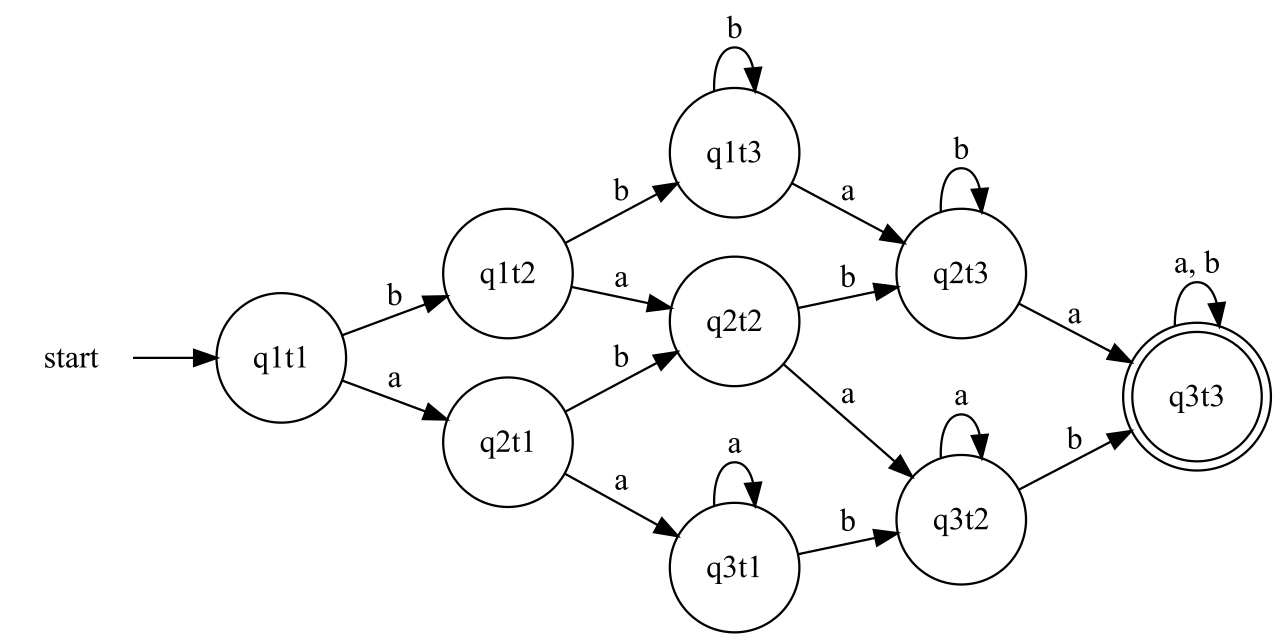
\includegraphics[scale = 1]{Task_2_1.png}
\caption{Задание № 2.1. Итоговый автомат.}
\end{figure}

\item$$ L_2 = \{\omega \in \{a, b\}^* \mid |\omega| \geq 3 \wedge |\omega| \, \text{нечётное} \} $$

\noindentПусть автомат A распознает следующий язык: $ L_{21} = \{\omega \in \{a, b\}^* \mid |\omega| \geq 3 \} $

\begin{figure}[!h]
\centering
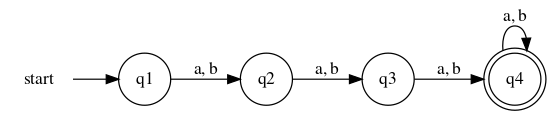
\includegraphics[scale = 0.8]{Task_2_21.png}
\caption{Задание № 2.2. Автомат A.}
\end{figure}

\noindentПусть автомат B распознает следующий язык: $ L_{22} = \{\omega \in \{a, b\}^* \mid |\omega| \, \text{нечётное} \} $

\begin{figure}[!h]
\centering
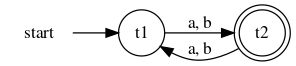
\includegraphics[scale = 0.8]{Task_2_22.png}
\caption{Задание № 2.2. Автомат B.}
\end{figure}

\noindentАвтомат A: $ \Sigma_1 = \{a, b\}$, $ Q_1 = \{q1, q2, q3, q4 \} $, q1 - н.ч., $ T_1 = \{q4 \} $, $ \delta_1 $ - ф.п.

\noindentАвтомат B: $ \Sigma_2 = \{a, b\}$, $ Q_2 = \{t1, t2\} $, t1 - н.ч., $ T_2 = \{t2 \} $, $ \delta_2 $ - ф.п.

\noindentРассмотрим прямое произведение 2-х автоматов.

\noindent$ \Sigma = \{a, b\}$

\noindent$ Q = \{q1t1, q1t2, q2t1, q2t2, q3t1, q3t2, q4t1, q4t2 \} $

\noindentНачальное состояние = q1t1

\noindent$ T = \{q4t2 \} $

\begin{center}
\begin{tabular}{ |c|c|c| } 
\hline
\, & a & b \\
\hline
 q1t1 & q2t2 & q2t2 \\
\hline
q1t2 & q2t1 & q2t1 \\
\hline
q2t1& q3t2 & q3t2 \\
\hline
q2t2 & q3t1 & q3t1 \\
\hline
q3t1 & q4t2 & q4t2 \\
\hline
q3t2 & q4t1 & q4t1 \\
\hline
q4t1 & q4t2 & q4t2 \\
\hline
q4t2 & q4t1 & q4t1 \\
\hline
\end{tabular}
\end{center}

\begin{figure}[!h]
\centering
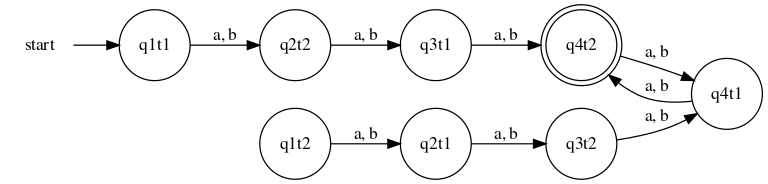
\includegraphics[scale = 0.6]{Task_2_2.png}
\caption{Задание № 2.2. Итоговый автомат.}
\end{figure}

\newpage

\noindentНачальное состояние в узле <<q1t1>>, поэтому невозможно попасть в узел <<q1t2>>, соответственно невозможно попасть в узлы <<q2t1>> и <<q3t2>>. Можем упростить данный ДКА.

\begin{figure}[!h]
\centering
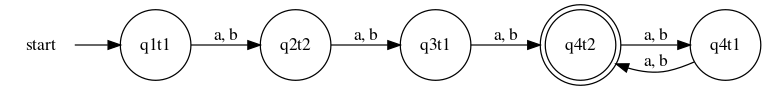
\includegraphics[scale = 0.6]{Task_2_2_other.png}
\caption{Задание № 2.2. Итоговый автомат (Упрощенный вариант).}
\end{figure}

\item$$ L_3 = \{\omega \in \{a, b\}^* \mid |\omega|_a \, \text{чётно} \wedge |\omega|_b \, \text{кратно трём} \} $$

\noindentРассмотрим каждое из условий по отдельности.

\noindentПусть автомат A распознает следующий язык: $ L_{31} = \{\omega \in \{a, b\}^* \mid |\omega|_a \, \text{чётно}\} $

\begin{figure}[!h]
\centering
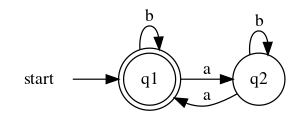
\includegraphics[scale = 0.7]{Task_2_31.png}
\caption{Задание № 2.3. Автомат A.}
\end{figure}

\noindentПусть автомат B распознает следующий язык: $ L_{32} = \{\omega \in \{a, b\}^* \mid |\omega|_b \, \text{кратно трём} \} $

\begin{figure}[!h]
\centering
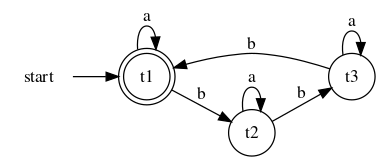
\includegraphics[scale = 0.6]{Task_2_32.png}
\caption{Задание № 2.3. Автомат B.}
\end{figure}

\noindentАвтомат A: $ \Sigma_1 = \{a, b\}$, $ Q_1 = \{q1, q2 \} $, q1 - н.ч., $ T_1 = \{q1 \} $, $ \delta_1 $ - ф.п.

\noindentАвтомат B: $ \Sigma_2 = \{a, b\}$, $ Q_2 = \{t1, t2, t3\} $, t1 - н.ч., $ T_2 = \{t1 \} $, $ \delta_2 $ - ф.п.

\noindentРассмотрим прямое произведение 2-х автоматов.

\noindent$ \Sigma = \{a, b\}$

\noindent$ Q = \{q1t1, q1t2, q1t3, q2t1, q2t2, q2t3\} $

\noindentНачальное состояние = q1t1

\noindent$ T = \{q1t1 \} $

\begin{center}
\begin{tabular}{ |c|c|c| } 
\hline
\, & a & b \\
\hline
 q1t1 & q2t1 & q1t2 \\
\hline
q1t2 & q2t2 & q1t3 \\
\hline
q1t3 & q2t3 & q1t1 \\
\hline
q2t1 & q1t1 & q2t2 \\
\hline
q2t2 & q1t2 & q2t3 \\
\hline
q2t3 & q1t3 & q2t1 \\
\hline
\end{tabular}
\end{center}

\begin{figure}[!h]
\centering
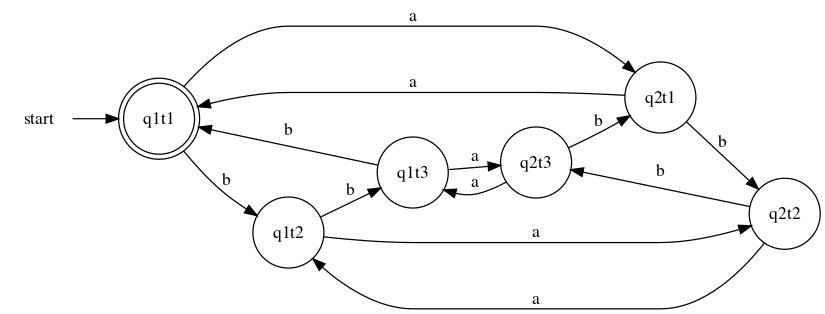
\includegraphics[scale = 0.55]{Task_2_3.png}
\caption{Задание № 2.3. Итоговый автомат.}
\end{figure}

\item$$ L_4 = \overline L_3 $$

\noindent$ \Sigma = \{a, b\}$

\noindent$ Q = \{q1t1, q1t2, q1t3, q2t1, q2t2, q2t3\} $

\noindentНачальное состояние = q1t1

\noindent$ T = \{q1t2, q1t3, q2t1, q2t2, q2t3 \} $

\begin{center}
\begin{tabular}{ |c|c|c| } 
\hline
\, & a & b \\
\hline
 q1t1 & q2t1 & q1t2 \\
\hline
q1t2 & q2t2 & q1t3 \\
\hline
q1t3 & q2t3 & q1t1 \\
\hline
q2t1 & q1t1 & q2t2 \\
\hline
q2t2 & q1t2 & q2t3 \\
\hline
q2t3 & q1t3 & q2t1 \\
\hline
\end{tabular}
\end{center}

\begin{figure}[!h]
\centering
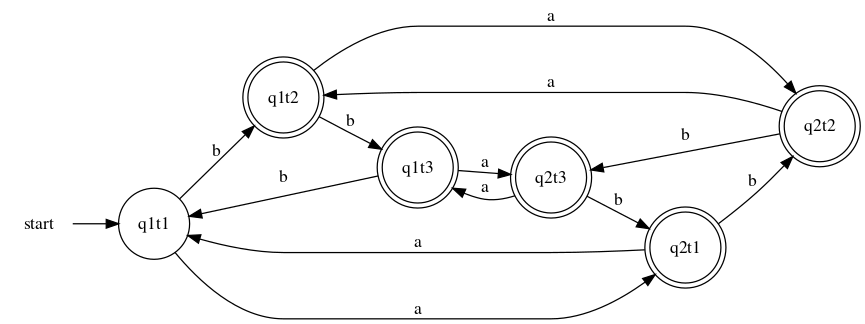
\includegraphics[scale = 0.55]{Task_2_4.png}
\caption{Задание № 2.4. Итоговый автомат.}
\end{figure}

\item$$ L_5= L_2 \setminus L_3 $$
$$ L_5= L_2 \setminus L_3 = L_2 \cap \overline L_3 = L_2 \cap L_4 $$

\noindentПусть автомат A распознает язык $L_2$.

\begin{figure}[!h]
\centering
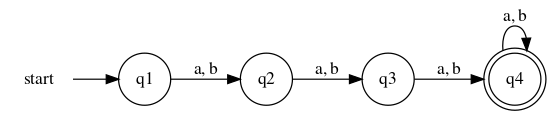
\includegraphics[scale = 0.8]{Task_2_51.png}
\caption{Задание № 2.5. Автомат A.}
\end{figure}

\noindentПусть автомат B распознает язык $L_4$.

\begin{figure}[!h]
\centering
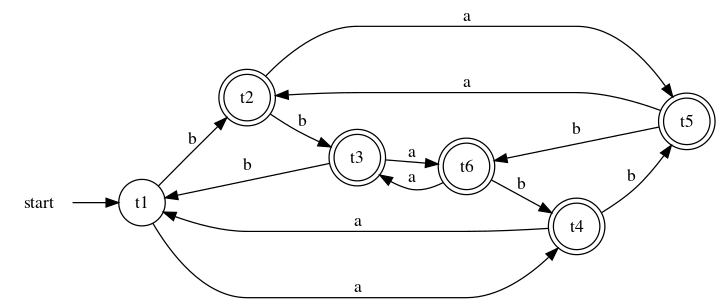
\includegraphics[scale = 0.6]{Task_2_52.png}
\caption{Задание № 2.5. Автомат B.}
\end{figure}

\noindentАвтомат A: $ \Sigma_1 = \{a, b\}$, $ Q_1 = \{q1, q2, q3, q4 \} $, q1 - н.ч., $ T_1 = \{q4 \} $, $ \delta_1 $ - ф.п.

\noindentАвтомат B: $ \Sigma_2 = \{a, b\}$, $ Q_2 = \{t1, t2, t3. t4. t5. t6\} $, t1 - н.ч., $ T_2 = \{t2, t3, t4, t5, t6 \} $, $ \delta_2 $ - ф.п.

\noindentРассмотрим прямое произведение 2-х автоматов.

\noindent$ \Sigma = \{a, b\}$

\noindent$ Q = \{q1t1, q1t2, q1t3, q1t4, q1t5, q1t6, q2t1, q2t2, q2t3, q2t4, q2t5, q2t6, q3t1, q3t2, q3t3,$

$ q3t4, q3t5, q3t6, q4t1, q4t2, q4t3, q4t4, q4t5, q4t6\} $

\noindentНачальное состояние = q1t1

\noindent$ T = \{q4t2, q4t3, q4t4, q4t5, q4t6 \}$

\begin{center}
\begin{tabular}{ |c|c|c| } 
\hline
\, & a & b \\
\hline
q1t1 & q2t4 & q2t2 \\
\hline
q1t2 & q2t5 & q2t3 \\
\hline
q1t3 & q2t6 & q2t1 \\
\hline
q1t4 & q2t1 & q2t5 \\
\hline
q1t5 & q2t2 & q2t6 \\
\hline
q1t6 & q2t3 & q2t4 \\
\hline

q2t1 & q3t4 & q3t2 \\
\hline
q2t2 & q3t5 & q3t3 \\
\hline
q2t3 & q3t6 & q3t1 \\
\hline
q2t4 & q3t1 & q3t5 \\
\hline
q2t5 & q3t2 & q3t6 \\
\hline
q2t6 & q3t3 & q3t4 \\
\hline

q3t1 & q4t4 & q4t2 \\
\hline
q3t2 & q4t5 & q4t3 \\
\hline
q3t3 & q4t6 & q4t1 \\
\hline
q3t4 & q4t1 & q4t5 \\
\hline
q3t5 & q4t2 & q4t6 \\
\hline
q3t6 & q4t3 & q4t4 \\
\hline

q4t1 & q4t4 & q4t2 \\
\hline
q4t2 & q4t5 & q4t3 \\
\hline
q4t3 & q4t6 & q4t1 \\
\hline
q4t4 & q4t1 & q4t5 \\
\hline
q4t5 & q4t2 & q4t6 \\
\hline
q4t6 & q4t3 & q4t4 \\
\hline

\end{tabular}
\end{center}

\begin{figure}[!h]
\centering
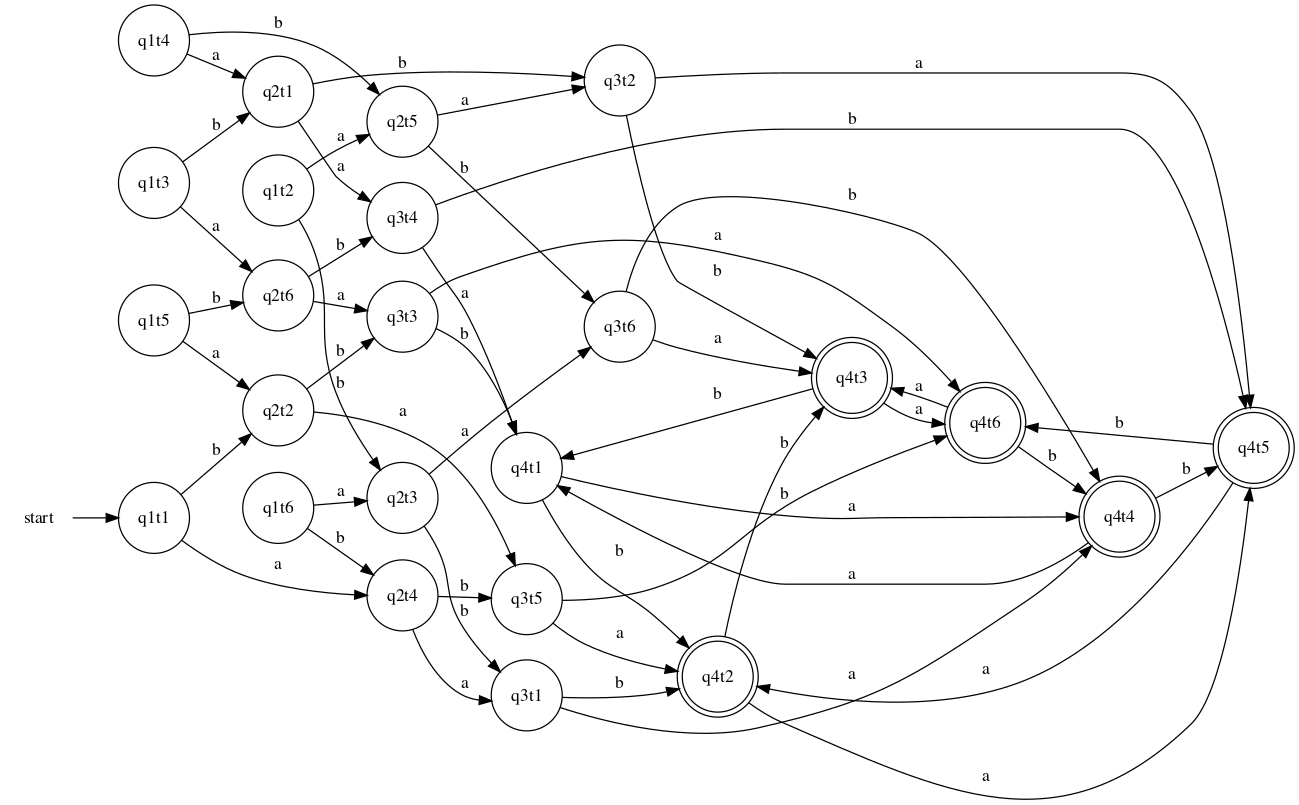
\includegraphics[scale = 0.38]{Task_2_5.png}
\caption{Задание № 2.5. Итоговый автомат.}
\end{figure}

\end{enumerate}

\newpage

\section{Задание № 3. Построить минимальный ДКА по регулярному выражению.}

Ответом на данное задание является минимальный ДКА, который допускает тот же язык, что описывается регулярным выражением.

\begin{enumerate}

\item$(ab + aba)^*a$ 

\noindentПостроим НКА:

\begin{figure}[!h]
\centering
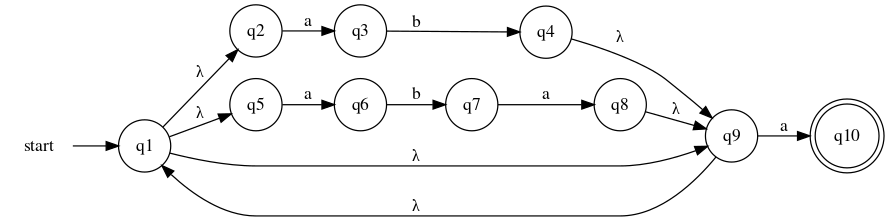
\includegraphics[scale = 0.5]{NKA_3_1.png}
\caption{Задание № 3.1. НКА.}
\end{figure}

\noindentПостроим ДКА:

\begin{center}
\begin{tabular}{ |c|c|c| } 
\hline
\, & a & b \\
\hline
 \{q1\} & \{q3, q6, q10\} & $\varnothing$\\
\hline
 \{q3, q6, q10\} & $\varnothing$ & \{q4, q7\} \\
\hline
 \{q4, q7\} & \{q3, q6, q8, q10\} & $\varnothing$\\
\hline
 \{q3, q6, q8, q10\} &  \{q3, q6, q10\} &  \{q4, q7\} \\
\hline
\end{tabular}
\end{center}

\begin{figure}[h!]
\centering
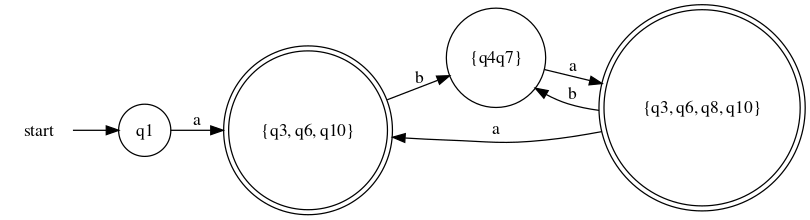
\includegraphics[scale = 0.5]{DKA_3_1.png}
\caption{Задание № 3.1. ДКА.}
\end{figure}

Полученный ДКА является минимальным.

\item$ a(a(ab)^*b)^*(ab)^* $ 

\noindentПостроим НКА:

\begin{figure}[h!]
\centering
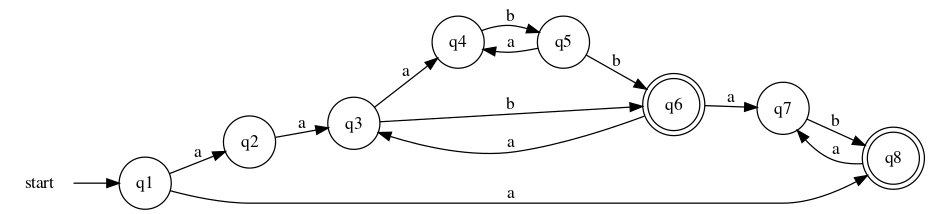
\includegraphics[scale = 0.5]{NKA_3_2.png}
\caption{Задание № 3.2. НКА.}
\end{figure}

\begin{center}
\begin{tabular}{ |c|c|c| } 
\hline
\, & a & b \\
\hline
 \{q1\} & \{q2, q8\} & $\varnothing$ \\
\hline
 \{q2, q8\} & \{q3, q7\} & $\varnothing$ \\
\hline
 \{q3, q7\} & \{q4\} & \{q6, q8\} \\
\hline
 \{q4\} & $\varnothing$ &  \{q5\} \\
\hline
 \{q6, q8\} & \{q3, q7\} & $\varnothing$ \\
\hline
 \{q5\} & \{q4\} & \{q6\} \\
\hline
 \{q6\} & \{q3, q7\} & $\varnothing$ \\
\hline
\end{tabular}
\end{center}

\begin{figure}[h!]
\centering
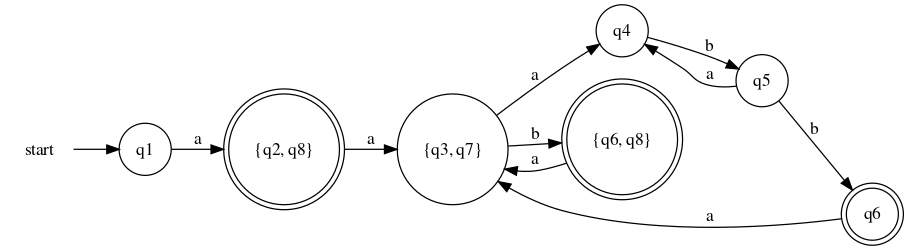
\includegraphics[scale = 0.5]{DKA_3_2.png}
\caption{Задание № 3.2. ДКА.}
\end{figure}

\noindentПостроим минимальный ДКА:

\noindent0 эквивалентность: (q1, q3q7, q4, q5), (q2q8, q6q8, q6)

\noindent1 эквивалентность: (q1), (q3q7, q5), (q4), (q2q8, q6q8, q6)

\begin{figure}[h!]
\centering
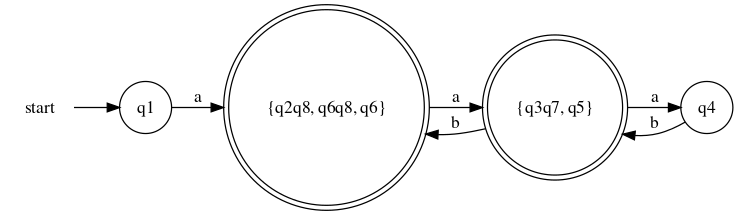
\includegraphics[scale = 0.6]{DKA_3_2_min.png}
\caption{Задание № 3.2. Минимальный ДКА.}
\end{figure}

\item $ (a+(a+b)(a+b)b)^* $ 

\noindentПостроим НКА:

\begin{figure}[h!]
\centering
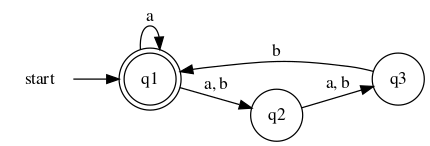
\includegraphics[scale = 0.6]{NKA_3_3.png}
\caption{Задание № 3.3. НКА.}
\end{figure}

\begin{center}
\begin{tabular}{ |c|c|c| } 
\hline
\, & a & b \\
\hline
 \{q1\} & \{q1, q2\} & \{q2\} \\
\hline
 \{q1, q2\} & \{q1, q2, q3\} & \{q2, q3\} \\
\hline
 \{q2\} & \{q3\} & \{q3\} \\
\hline
 \{q1, q2, q3\} & \{q1, q2, q3\} & \{q1, q2, q3\} \\
\hline
 \{q2, q3\} & \{q3\} & \{q1, q3\} \\
\hline
 \{q3\} & $\varnothing$ & \{q1\} \\
\hline
 \{q1, q3\} & \{q1, q2\} & \{q1, q2\} \\
\hline
\end{tabular}
\end{center}

\begin{figure}[h!]
\centering
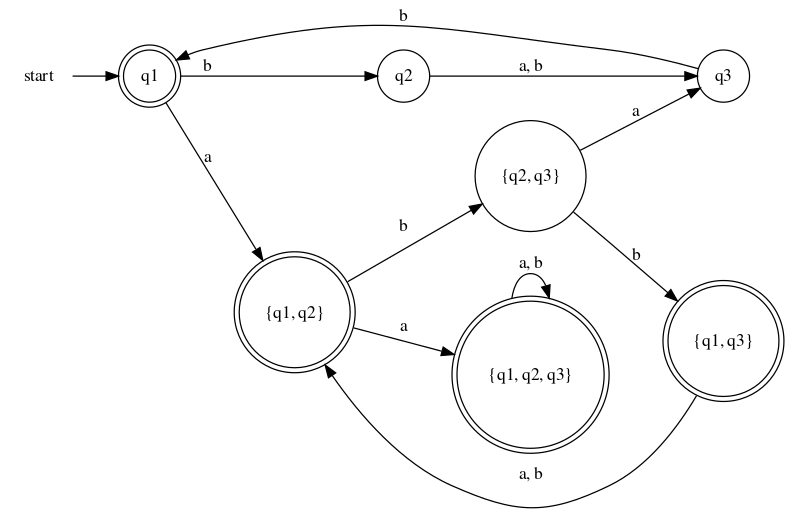
\includegraphics[scale = 0.5]{DKA_3_3.png}
\caption{Задание № 3.3. ДКА.}
\end{figure}

Полученный ДКА является минимальным.

\item $ (b+c)((ab)^*c+(ba)^*)^* $ 

\noindentПостроим ДКА:

\begin{figure}[h!]
\centering
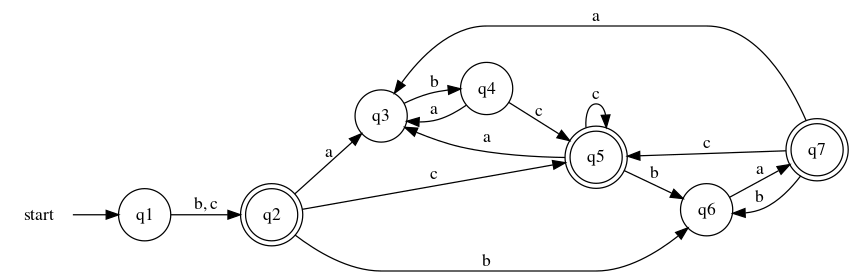
\includegraphics[scale = 0.6]{DKA_3_4.png}
\caption{Задание № 3.4. ДКА.}
\end{figure}

\noindentПостроим минимальный ДКА:

\noindent0 эквивалентность: (q1, q3, q4, q6), (q2, q5, q7)

\noindent1 эквивалентность: (q1) (q4), (q3), (q6), (q2q5q7)

\begin{figure}[h!]
\centering
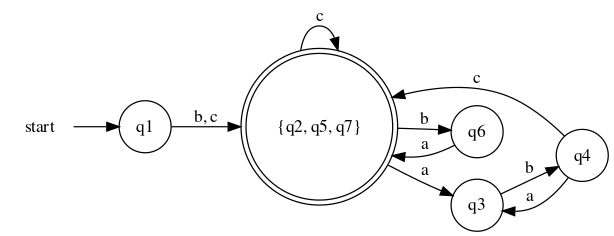
\includegraphics[scale = 0.6]{DKA_3_4_min.png}
\caption{Задание № 3.4. Минимальный ДКА.}
\end{figure}

\newpage

\item$ (a+b)^+(aa+bb+abab+baba)(a+b)^+ $ 

\noindentПостроим НКА:

\begin{figure}[h!]
\centering
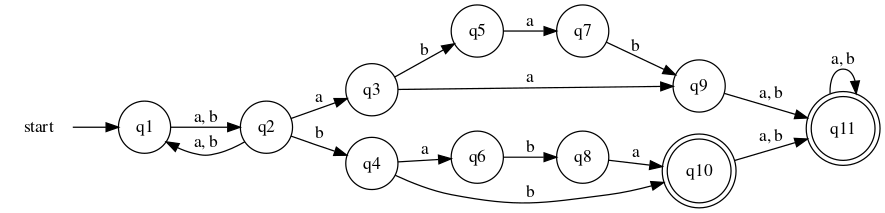
\includegraphics[scale = 0.5]{NKA_3_5.png}
\caption{Задание № 3.5. НКА.}
\end{figure}

\begin{center}
\begin{tabular}{ |c|c|c| } 
\hline
\, & a & b \\
\hline
 \{q1\} & \{q2\} & \{q2\} \\
\hline
 \{q2\} & \{q1, q3\} & \{q1, q4\} \\
\hline
 \{q1, q3\} & \{q2, q9\} & \{q2, q5\} \\
\hline
 \{q1, q4\} & \{q2, q6\} & \{q2, q10\} \\
\hline
 \{q2, q9\} & \{q1, q3, q11\} & \{q1, q4, q11\} \\
\hline
 \{q2, q5\} & \{q1, q3, q7\} & \{q1, q4\} \\
\hline
 \{q2, q6\} & \{q1, q3\} & \{q1, q4, q8\} \\
\hline
\{q2, q10\} & \{q1, q3, q11\} & \{q1, q4, q11\} \\
\hline
\{q1, q3, q11\} & \{q2, q9, q11\} & \{q2, q5, q11\} \\
\hline
\{q1, q4, q11\} & \{q2, q6, q11\} & \{q2, q10, q11\} \\
\hline
\{q1, q3, q7\} & \{q2, q9\} & \{q2, q5, q9\} \\
\hline
\{q1, q4, q8\} & \{q2, q6, q10\} & \{q2, q10\} \\
\hline
\{q2, q9, q11\} & \{q1, q3, q11\} & \{q1, q4, q11\} \\
\hline
\{q2, q5, q11\} & \{q1, q3, q7, q11\} & \{q1, q4, q11\} \\
\hline
\{q2, q6, q11\} & \{q1, q3, q11\} & \{q1, q4, q8, q11\} \\
\hline
\{q2, q10, q11\} & \{q1, q3, q11\} & \{q1, q4, q11\} \\
\hline
\{q2, q5, q9\} & \{q1, q3, q7, q11\} & \{q1, q4, q11\} \\
\hline
\{q2, q6, q10\} & \{q1, q3, q11\} & \{q1, q4, q8, q11\} \\
\hline
\{q1, q3, q7, q11\} & \{q2, q9, q11\} & \{q2, q5, q9, q11\} \\
\hline
\{q1, q4, q8, q11\} & \{q2, q6, q10, q11\} & \{q2, q10, q11\} \\
\hline
\{q2, q5, q9, q11\} & \{q1, q3, q7, q11\} & \{q1, q4, q11\} \\
\hline
\{q2, q6, q10, q11\} & \{q1, q3, q11\} & \{q1, q4, q8, q11\} \\
\hline
\end{tabular}
\end{center}

\begin{figure}[h!]
\centering
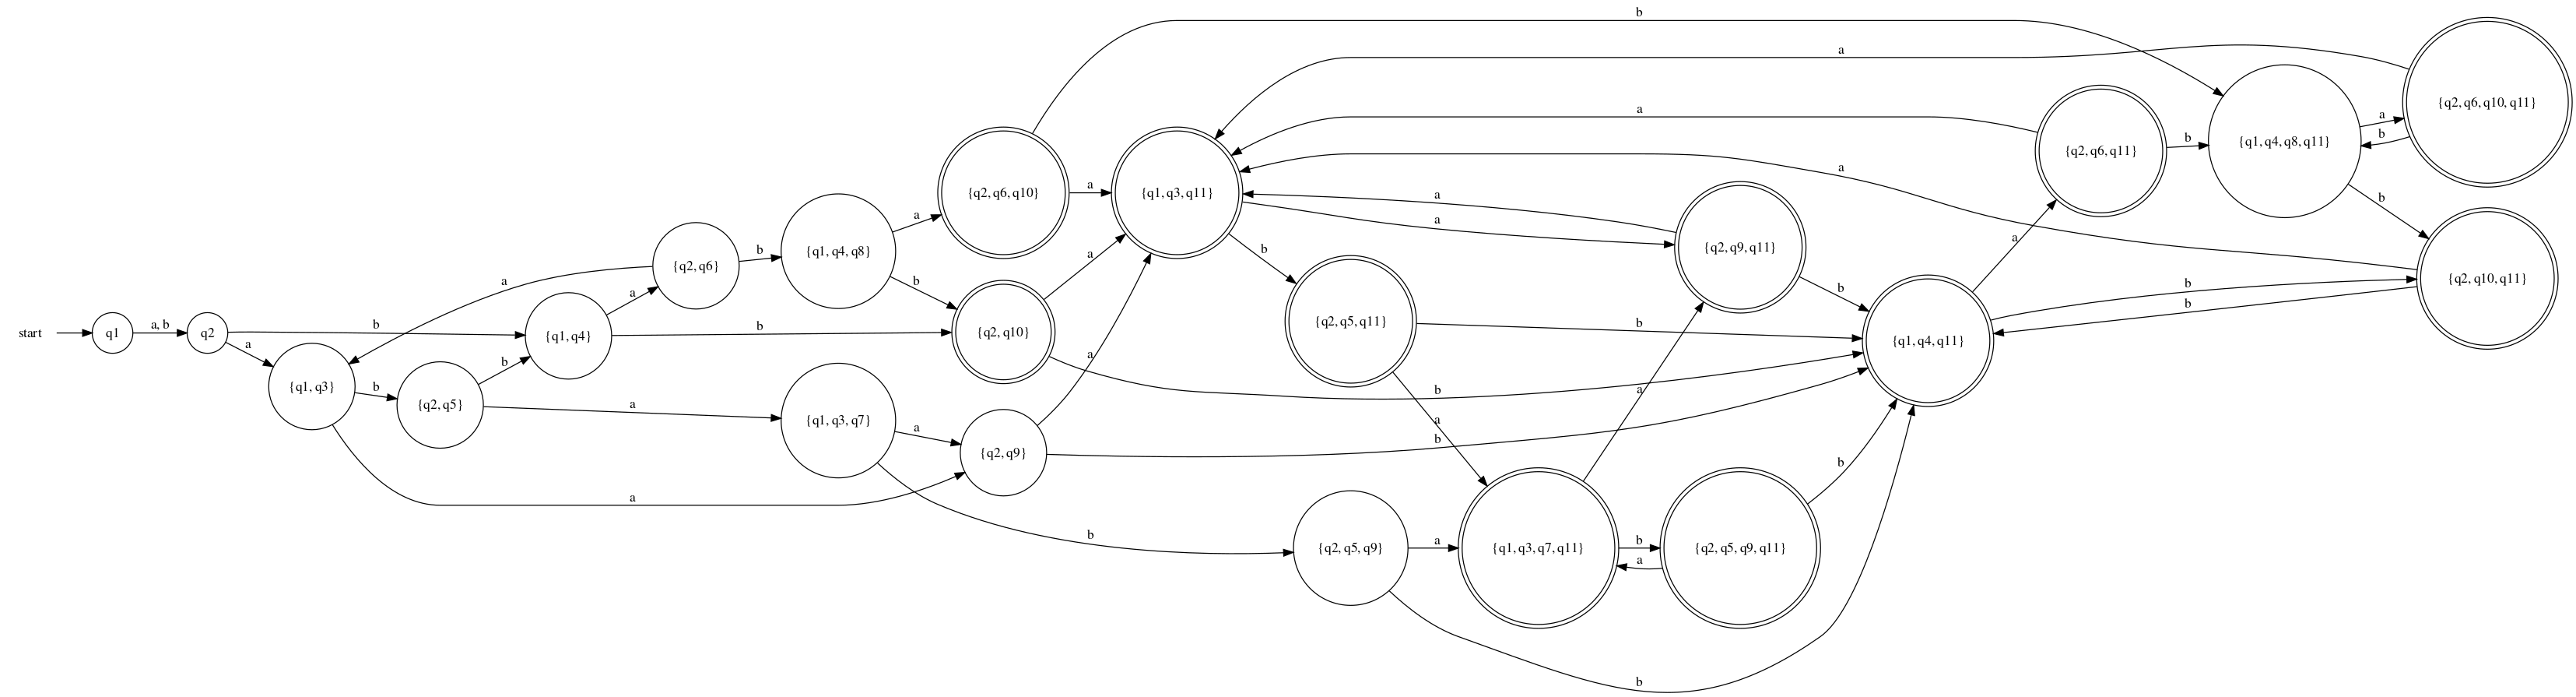
\includegraphics[scale = 0.15]{DKA_3_5.png}
\caption{Задание № 3.5. ДКА.}
\end{figure}

\noindent0 эквивалентность: (q1, q2, q1q3, q1q4, q2q9, q2q5, q2q6, q1q3q7, q1q4q8, q2q5q9), (q2q10, q1q3q11, q1q4q11, q2q9q11, q2q5q11, q2q6q11, q2q10q11, q2q6q10, q1q3q7q11, q1q4q8q11, q2q5q9q11, q2q6q10q11)

\end{enumerate}

\section{Задание № 4. Определить, является ли язык регулярным или нет.}

Ответом на данное задание является конечный автомат, если язык регулярен, либо доказательство нерегулярности языка при помощи леммы о разрастании.

\begin{enumerate}

\item$$ L = \{(aab)^nb(aba)^m \mid n \geq 0, m \geq 0 \} $$

\begin{figure}[h!]
\centering
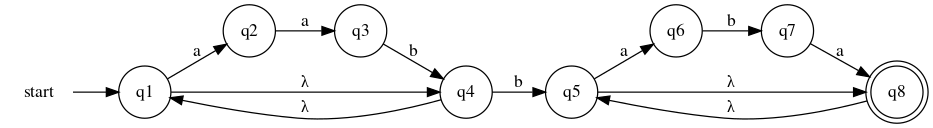
\includegraphics[scale = 0.5]{KA_4_1.png}
\caption{Задание № 4.1. Конечный автомат.}
\end{figure}

\noindentДанный язык является регулярным.

\item$$L = \{ uaav \mid u \in \{a, b\}^*, v \in \{a, b\}^*, |u|_b \geq |v|_a \}$$

\noindentИспользуем лемму о разрастании.

\noindentПусть L - это регулярный язык. Тогда 

$ \exists n \, \forall w \in L, |w| \geq n \,\exists x, y, z \, w=xyz \, |xy| \leq n \,  y \neq \varepsilon \, \forall i \geq 0 \, xy^iz \in L. $ 

\noindentОтрицание:

\noindent$ \forall n \, \exists w \in L, |w| \geq n \, \forall x, y, z \, w=xyz \, |xy| \leq n \,  y \neq \varepsilon \, \exists i \geq 0 \, xy^iz \notin L. $

\noindentРассмотрим слово: $ \omega = b^naaa^n, |\omega| \geq n $
$$ \omega = xyz $$
$$ x = b^i, \quad y=b^j \quad i + j \leq n \quad j > 0 $$
$$ |xy| \leq n \quad |y| > 0 $$
$$ z = b^{n-i-j}aaa^n $$
$$ xy^0z = b^ib^{n-i-j}aaa^n = b^{n-j}aaa^n\notin L $$

\noindentЧ.т.д. Язык является не регулярным языком.

\item$$L = \{ a^mw \mid w \in \{a, b\}^*, 1 \leq |w|_b \leq m \}$$

\noindentРассмотрим слово: $ \omega = a^mb^m, |\omega| \geq m $
$$ \omega = xyz $$
$$ x = a^i, \quad y=a^j \quad i + j \leq m \quad j > 0 $$
$$ |xy| \leq m \quad |y| > 0 $$
$$ a^{m-i-j}b^m $$
$$ xy^0z = a^ia^{m-i-j}b^m = a^{m-j}b^m \notin L, \text{т.к.} j \neq 0$$

\noindentЧ.т.д. Язык является не регулярным языком.

\item$$L = \{ a^kb^ma^n \mid k = n \vee m > 0 \}$$

\noindentРассмотрим слово: $ \omega = a^nba^n, |\omega| \geq n $
$$ \omega = xyz $$
$$ x = a^i, \quad y=a^j \quad i + j \leq n \quad j > 0 $$
$$ |xy| \leq n \quad |y| > 0 $$
$$ z=a^{n-i-j}ba^n $$
$$ xy^2z = a^ia^{2j}a^{n-i-j}ba^n = a^{n+j}ba^n \notin L, \text{т.к.} j \neq 0 $$

\noindentЧ.т.д. Язык является не регулярным языком.

\item$$L = \{ ucv \mid u \in \{a, b\}^*, v \in \{a, b\}^*, u \neq v^R \}$$

\noindentРассмотрим слово: $ \omega = (ab)^nc(ab)^n, |\omega| \geq n $
$$ \omega = (ab)^nc(ab)^n=\alpha_1\alpha_2...\alpha_{4n+1}, |\omega| \geq n $$
$$ \omega = xyz $$
$$ x = \alpha_1\alpha_2...\alpha_i, \quad y=\alpha_{i+1}\alpha_{i+2}...\alpha_{i+j} \quad i + j \leq n \quad j > 0 $$
$$ |xy| \leq n \quad |y| > 0 $$
$$ z=\alpha_{i+j+1}\alpha_{i+j+2}...\alpha_{2n}c(ab)^n $$
$$ xy^kz = \alpha_1...\alpha_i(\alpha_{i+1}...\alpha_{i+j})^k\alpha_{i+j+1}...\alpha_{2n}c(ab)^n \notin L \quad \forall k > 1 $$

\noindentЧ.т.д. Язык является не регулярным языком.

\end{enumerate}

\end{document}
